\documentclass[6pt]{article}
\usepackage{geometry}                % See geometry.pdf to learn the layout options. There are lots.
\geometry{letterpaper}                   % ... or a4paper or a5paper or ... 
%\geometry{landscape}                % Activate for for rotated page geometry
%\usepackage[parfill]{parskip}    % Activate to begin paragraphs with an empty line rather than an indent
\usepackage{graphicx}
\usepackage{amssymb}
\usepackage{epstopdf}
\usepackage{tipa}
\usepackage{amsmath}
\usepackage{floatrow}
\usepackage{subcaption}


\DeclareGraphicsRule{.tif}{png}{.png}{`convert #1 `dirname #1`/`basename #1 .tif`.png}
\graphicspath{{/Users/marlon/Documents/BA/thesis/pictures/}}

\title{Unsupervised Cognate Identification with Variational Autoencoders}
\author{Marlon Betz}
%\date{}                                           % Activate to display a given date or no date

\begin{document}
\maketitle
\newpage
\tableofcontents
\newpage

\section{Introduction}

Historical Linguistics investigates language from a diachronic perspective, i.e. it seeks to uncover the history of languages and the structure of the hidden forces that drive language change.  Computational Historical Linguistics accordingly deals with computational methods to explore the history of languages and topics closely related to it, such as phylogenetic inferences of language families \cite{bouckaert2012mapping}, migration of language speakers \cite{gray2009language}, inferring lexical flows between languages \cite{dellert2015uralic} or modeling sound change \cite{bouchard2013automated}.  

On the other hand, deep neural networks have been proven to uncover latent features of data and use them for a variety of tasks, such as computer vision or various NLP tasks, e.g. Document classification, Sentiment Analysis or Speech synthesis. 

Bayesian Hierarchical models have been proven to allow for a detailed analysis of data and testing hypotheses in the fields of Psycholinguistics. In fact, Bayesian models build the backbone for most phylogenetic surveys.

Over the past few years, deep neural networks have been interconnected with Bayesian methods in the form of Deep Generative Models. They combine the strength of deep networks to uncover latent features with the power of bayesian inference. Today, deep generative models are the main object of current AI research. 

 However, Computational Historical Linguistics has hardly been touched yet by the current Deep Learning boom (a notable exception is \cite{rama2016siamese}). 
 In fact, most computational models here are either adaptations or direct copies of those used for the description of biological data.
The aim of this thesis is hence 
\begin{enumerate}
\item to combine methods from both Computational Historical Linguistics, Bayesian Models and the emerging field of Deep Learning
\item to propose a model of modeling sound change as a walk in latent space, which is suitable for neural networksand builds the basis for this thesis
\item to use variational autoencoders as a means to build such a latent space, and to investigate it
\item to show how this uncovered structure can be used to identify cognates in an unsupervised way
\end{enumerate}

I will first start by giving an overview of the problem of cognate identification and related fields of research. I will give a background on why cognate identification is important to discuss the historical connections between languages and further provide an overview on several established methods to detect cognates.  

Then I will proceed to introduce the concept of sound change as a walk in latent space, which serves as a background for the actual inference model. Here I will talk about the main motivations for this approach as well as its major drawbacks. 


I will then discuss the actual architecture of the inference model. This first covers a general overview on the components included in the model. I will then in detail look over all components in particular. That will first cover a discussion of different methods of phoneme vectorizations. This is followed by a general overview on autoencoders as non-linear dimensionality reduction architectures first and then a description of variational autoencoders in particular, which build the basis for the model described here. I then come to the discussion of possible ways to cluster the words, i.e. to assign the actual inferred cognacy labels.

Then I will document how well those methods can be used to infer cognacy between words. I will compare the inferred labels with expert judgements first and then see how the inferred labels can infer language phylogenies, using both neighbor joining and established bayesian models of cognate evolution.

Finally, I will give a resume on the model described here.


\section{Sound Change as a Walk in Latent Space}
\label{Sound Change as a Walk in Latent Space}
\subsection{Motivation}

\begin{figure}[h]
\begin{center}
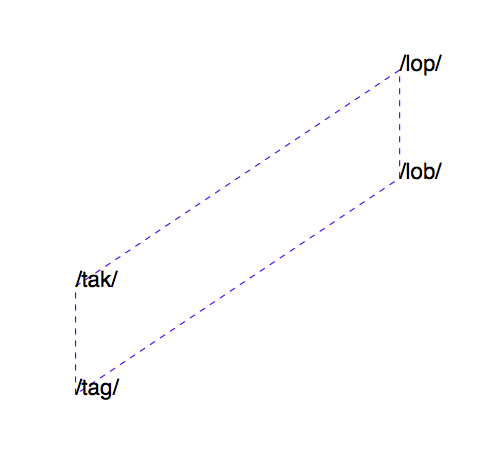
\includegraphics[width=0.5\textwidth]{sc_fake_example} 
\caption{Visualization of the concept of sound change as a walk in latent space. Here, sound changes are vectors from one word to another, where both word forms are given as points in latent space. The vector from /lob/ to /lop/ would be the same as from /tag/ to /tak/, as both vectors would describe the loss of voice in the word-final phoneme. This linear dependence means that if we fit a regression model from /tag/ to /tak/, we could generalize well to predict /lop/ from /lob/. The different lengths of the vectors are than proportional to probabilities of such as sound change to appear. Here, final devoicing should be more probable than a change from /lop/ to /tak/. }
\label{default}
\end{center}
\end{figure}
In linguistic literature, sound change is usually described as a change of distinctive phonological features over phonological symbols. For instance, a sound change such as final devoicing as in 

\begin{equation}
MHG /hund/ \rightarrow NHG /hunt/
\end{equation}

 would be captured by an string edit rule like
\begin{equation}
/d/ \rightarrow /t/ / \_ \#
\end{equation}

that says that /d/ becomes /t/ before the end of a word. Such sound changes are shown not to appear randomly, but to co-occur according to some latent features. E.g. a sound change like above should leave the language without final /d/, while final /b/ and /g/ would be allowed. Such situations are evolutionary highly unstable, so we would expect the other voiced plosives to change to /p/ and /k/ accordingly. This is due to latent phonological features such as \textsc{[voice]}, \textsc{[labial]} or \textsc{[ATR]}, which are usually described to appear either in a binary or privative feature space. Accordingly, our rule from above could be generalized to

\begin{equation}
\textsc{[+voice]} \rightarrow \textsc{[-voice]} / \_ \#
\label{eq:final_devoicing}
\end{equation}
which describes the loss of voice at the end of a word. 

Computational models of sound change usually treat words as string of symbols and sound change as substitution of substrings.\cite{bouchard2007probabilistic,bouchard2013automated} use a generative model that learns to substitute substrings in some latent order and achieve good performances on the reconstruction of ancient forms of words as well as on cognate identification. However, such a method has two major drawbacks: On the one hand, it needs the topology of the languages phylogeny to be known beforehand. This problem does not exist for certain language families with established tree topologies, but can be problematic if language relationships are not totally clear. On the other hand, such purely symbolic models need lot of data to generalize well. \cite{bouchard2007probabilistic} for example underline that their model cannot model chain shifts as such.

This thesis proposes a model that tries to solve the task of cognate identification (and sound change as such) under the following assumptions:
\begin{enumerate}
\item The functions connecting our data with some latent space should be smooth. This allows the model to generalize from training examples to nearby points in input space, even if they were not trained on.
\item The relationships between the data can be explained by some linear function, i.e. the data is linearly dependent. This should allow for good predictions even when the test data is far away from the training data.
\item The underlying linear factors that produce the data are to complex to model directly, but only exist in some latent space that is not directly visible. 
\item The model should treat factors that change some latent representation as causes for variation of the actual data, not vice versa.
\end{enumerate}

To address the smoothness assumption, we have to make sure that such a model treats phonemes and words not as symbols, but as points or distributions in some latent space. This allows for some tokens to be inherently closer to each other. \ref{Phoneme Vectorization} will discuss several such embedding methods for phonemes and \ref{Word Embeddings} will explore variational autoencoders as the preferred embedding algorithms for words.  




%Coming from rules that use distinctive phonological features as in Eq. \ref{eq:final_devoicing}, we can encode every word as a sequence of phonemes that are points in some phonological feature space $\mathcal{F}$, where each dimension corresponds to phonological features such as \textsc{[velar]} or \textsc{[approximant]}. 

The linearity assumption allows for the generalization over the compositional character of latent features over phonemes and words. For instance, in such a latent feature space $\mathcal{Z}$ over $\mathbb{R}^n$, a sound change $sc$ that derives a recent form of word $w_{recent}$ from an ancient form  $w_{ancient}$ should then correspond to a vector $v_{sc}$ in such a way that 
\begin{equation}
\label{eq:sound_change_linear_dependency}
v_{w_{ancient}}+v_{sc} = v_{w_{recent}}
\end{equation}

From this follows that 

\begin{equation}
v_{sc} =  v_{w_{recent}} - v_{w_{ancient}} 
\end{equation}

That is, we can formulate sound changes such as \ref{eq:final_devoicing} without neither the actual sound change nor the conditioning specifying where the sound change should apply, but only the respective words involved.
If we further assume that that sound change affects another word $w'$, we have

\begin{equation}
v_{w_{recent}} - v_{w_{ancient}}  =  v_{w'_{recent}} - v_{w'_{ancient}} 
\end{equation}
which is equivalent to
\begin{equation}
v_{w_{recent}}  =   v_{w_{ancient}}  + (v_{w'_{recent}} - v_{w'_{ancient}}) 
\end{equation}
If we want to evaluate that latent feature space, we investigate in how far that compositional structure is preserved in our latent space. In fact, such analogy tasks can be used as an evaluation method to test whether the learned embedding space encodes the structure expected to be inherently contained in the data (cf. \cite{mikolov2013distributed}).

\subsection{$P(z)$ as Prior for Evolutionary Stable Phoneme sequences}

The question is then how to construct such a latent space $\mathcal{Z}$. If we follow the assumption from above that the model should treat factors in latent space as causes for variation of the actual data and not vice versa and if we further know that all words share a common structure, such as syllables and their respective internal structure, we can assume that it should be possible to model that structure by a latent variable $z$ embedded in latent space. As $z$ walks through $\mathcal{Z}$, we assume that the resulting word $x$ changes in a \textit{meaningful} way - for instance it should change certain phonological features of some phonemes in $x$ given that such changes are plausible, given the context of the other phonemes in the words. It should also be possible to add whole new affixes, but it should not inherit implausible phoneme sequences or change phoneme features in some random way. 


As we expect that it is not possible to model the underlying factors that create the data directly, a decoder distribution $Q(z|X)$ cannot be mono-modal. However, we assume $Q(z|X)$ can be approximated by some universal function approximator that is combined with a stochastic unit. This multi-modality leads to the situation that similar points in $\mathcal{Z}$ should not necessarily coincide with similar points in our data space $\mathcal{X}$. For instance, a fictional word such as /aban/ should be closer to /ov\textipa{\~a}/ than to /a\textipa{\textdoublebarpipe}an/ in $\mathcal{Z}$ but not necessarily in $\mathcal{X}$, as it should be more probable that intervocalic voiced plosives lenite to fricatives and syllable-final nasals drop but leave some compensatory nasalization - here even at the same time - but there should be hardly any evidence of a direct sound change from /b/ to a palatal click.

%As we expect that it is not possible to model the underlying factors that create the data directly, a decoder function such as $f_{decode}:\mathcal{Z} \rightarrow \mathcal{X}$ cannot be linear. However, we assume $f_{decode}$ can be approximated by some universal function approximator.
%This non-linearity leads to the situation that similar points in $\mathcal{Z}$ should not necessarily coincide with similar points in our data space $\mathcal{X}$. For instance, a fictional word such as /aban/ should be closer to /ov\textipa{\~a}/ than to /a\textipa{\textdoublebarpipe}an/ in $\mathcal{Z}$ but not necessarily in $\mathcal{X}$, as it should be more probable that intervocalic voiced plosives lenite to fricatives and syllable-final nasals drop but leave some compensatory nasalization - here even at the same time - but there should be hardly any evidence of a direct sound change from /b/ to a palatal click.
%Moreover, as we are interested in modeling our latent features as as probabilistic variable, we are interested in an encoder distribution $Q(z|X)$ that models the probability of $z$ given our data $X$. For the reasons given above, we expect that distribution to be highly multimodal.

%
%To model the posterior $P(z|X)$, we can use Bayes' theorem:
%
%\begin{equation}
%P(z|X) = \frac{P(z)P(X|z)}{\int P(z)P(X|z)dz}
%\end{equation}
%
%Here, $P(z)$ is the prior probability of $z$ and $P(X|z)$ the likelihood of our data given our latent variable. The term in the denominator is the marginal probability $P(X)$ of our Data under the given model.
%If we want to model $z$ with the help of $X$, our objective is to maximize that marginal probability of our word list $P(X):
%
%\begin{equation}
%P(X) = \int P(z)P(X|z)dz
%\end{equation}
%
%

We further assume that a corresponding decoder distribution $P(X|z)$ can be modeled with the same means as $Q(z|X)$.  Both can consist of any distribution with continuous parameters, as they should be differentiable to allow for the backpropagation of error gradients through the model. 
%However, if our aim is to arrive with local modes in our posterior where evolutionary stable word forms that are similar to each other cluster among each other, we can assume that a given word $w$ in $\mathcal{Z}$ can be seen as some noisy version of another word $w'$ that is close to $w$ in $\mathcal{Z}$ - that is, we assume that $z$ can be modeled by a multivariate normal distribution. Mean and covariance of that distribution are than inferred by the model. Hence we further need a family of functions $f : \mathcal{Z} \times  \Theta \rightarrow \mathcal{X}$ that maps points in $\mathcal{Z}$ to points in the parameter space $\Theta$ of that normal distribution. The probability of our data given $z$ then becomes
%
%\begin{equation}
%P(X|z;\theta) = \mathcal{N}(X|f(z,\theta))
%\end{equation}

As we expect that the words in our word list follow the central limit theorem and in the long run should be captured by a normal distribution, our latent variable $z$ is sampled from a isotropic multivariate normal prior:
\begin{equation}
z \sim \mathcal{N}(0,I)
\end{equation}

where $I$ is the identity matrix.

If we train a deep probabilistic model such as variational autoencoders to approximate $Q(z|X)$ to $P(X)$ and maximize $P(X|z)$ (see \ref{Variational Autoencoders}), we can construct $\mathcal{Z}$ with the desired features. To arrive at such linear dependencies as in Eq. \ref{eq:sound_change_linear_dependency}, we then just have to expect them in our data $X$ in some way - e.g in form of predefined phoneme features as in \cite{kondrak2000new,list2012sca,rama2016siamese} that directly encode distinctive phonological features, pre-trained phoneme embeddings that capture the latent information of phonemes found in a corpus or as simple phoneme unigrams, in which case we would have the system learn latent phoneme features on its own. As $X$ in the decoder distribution $P(X|z)$ would be conditioned on $z$, we expect the same linear dependencies over words in $z$ as we find them in $X$.



%As we again do not directly know $P(w_{ancient}|w_{recent},z)$ nor $P(w_{ancient}|z)$ unless we have language-specific diachronic data to model that likelihood, we cannot directly infer $P(w_{recent}|w_{ancient},z)$. However, we can say that 
%\begin{equation}
%P(w_{ancient}|w_{recent},z) \propto P(w_{recent}|z) P(w_{recent}|w_{ancient},z)
%\end{equation}




During training, we expect the model to learn underlying features and exploit them. As a consequence, those features should be stored in $\mathcal{Z}$. As we expect that certain features are more salient than others and further apply a gaussian prior over $z$, this finally means that certain subspaces in $\mathcal{Z}$ also contain more encoded information than others. We can define that self-information $I(z)$ as
\begin{equation}
I(z) = - \log P(z)
\end{equation}
If we have a variable $C$ that defines the belief that a given sample of $z$ is a cognate to other words and hence shares latent features with other samples, we expect this belief into $C$ to be logarithmically proportional to the self-information of $z$, as $I(z)$ is also defined in log-space:
\begin{equation}
\begin{split}
\log P(C|z) & \propto  I(z) \\
\log P(C|z) & \propto  - \log P(z) \\
P(C|z) & \propto  - P(z) 
\end{split}
\end{equation}

This means that as the belief into $z$ \textit{decreases}, the belief that the given word is related to other words \textit{increases}. This negative proportionality is of great help: If we have two words $z_1$ and $z_2$ and both words share similar latent features and hence are located close to each other in $\mathcal{Z}$, but are both located in a subspace with high probability mass under our prior $P(X)$, our belief into a hypothetic common predecessor is much lower than if they were located in a subspace with low probability mass. Since we have a normal prior, this means inferred cognate clusters are pushed farer away from the center of $\mathcal{Z}$ the more evidence for their grouping exists. From this follows that words that have a low self-information are hence kept close to the center of $\mathcal{Z}$ and form a cluster on their own. If we recognize such a cluster in a subspace with high probability mass, we can be sure that the members of that cluster are words that do not have any cognates.
 
%However, this information-based interpretation of $P(Z)$ also means that we cannot assume that latent features that appear often during training also have a high probability in $\mathcal{Z}$.  



\subsection{Sound Change as Posterior $P(w_{recent}|w_{ancient},z)$ }


As we usually do not know the ancient version of a word but only recent ones, we expect the cognates to have spread through the latent space from the original ancient word form to some directions. Since we assume that bigger jumps from one point in $\mathcal{Z}$ are less likely than small ones, we can expect that recent versions of an ancient word form should still be in the vicinity of the ancient word. Under the simplifying assumption that words in our word list did not jump from one semantic concept to another, this allows us embed all words of a given semantic concept into $\mathcal{Z}$ and to cluster them.

However, there are some problems with this approach.
The actual distribution of recent word forms in $\mathcal{Z}$ given the ancient forms would be given by the posterior

\begin{equation}
P(w_{recent}|w_{ancient},z,X) = \frac{P(w_{recent})P(w_{ancient},z,X|w_{recent})}{\int P(w_{recent})P(w_{ancient},z,X|w_{recent})dw_{recent}}
\end{equation}

Unfortunately, we only know $P(w_{recent}|z,X)$, while we do not know $P(w_{ancient}|w_{recent},z,X)$ directly, i.e. we cannot say anything specific about the likelihood of an ancient word given the recent words, that is the distribution of probabilities over points in $\mathcal{Z}$ where an ancient word form could be, given the distribution of its own child words.
However, if we only consider those two terms and ignore the normalizing constant in the denominator, we have
\begin{equation}
P(w_{recent}|w_{ancient},z,X) \propto P(w_{recent}|z,X)P(w_{ancient}|w_{recent},z,X)
\end{equation}

This means that if our prior $P(w_{recent}|z,X)$, which is known to us, has low probability density for the area around $w_{recent}$, we can be quite certain that $P(w_{recent}|w_{ancient},z,X)$ should also be in such a low probability density area. As we except that the likelihood  $P(w_{ancient}|w_{recent},z)$ itself prefers points in $\mathcal{Z}$ that are close to $w_{recent}$ over points that are far away from it, we can say that $w_{recent}$ should be close to $w_{ancient}$. 
However, if our prior $P(w_{recent}|z,X)$ is in an area with high probability density, the likelihood does not have such a regulating effect, as the high prior probability would allow for many points in Z to a possible point for $w_{ancient}$. 
That has two major implications:


\begin{itemize}
\item  If we unpack our known prior $P(w_{recent}|z,X)$, we have
\begin{equation}
\begin{split}
P(w_{recent}|z,X)  & = \frac{P(w_{recent})P(z,X|w_{recent})}{P(z,X)} \\
P(w_{recent}|z,X) & \propto P(w_{recent})P(z,X|w_{recent})\\
P(w_{recent}|z,X) & \propto P(w_{recent})\frac{P(z,X)P(w_{recent}|X,z)}{P(w_{recent})}\\
P(w_{recent}|z,X) & \propto P(z,X)P(w_{recent}|z,X)\\
P(w_{recent}|z,X) & \propto P(X)P(z|X)P(w_{recent}|z,X)\\
\end{split}
\end{equation}
which involves the marginal probability of our data $P(X)$. If our data is small,  we assume that most words do not look similar. 
For example, if we image that we have a word such as  /o/, we can hardly make any claims about how some ancient form would look like - it could come from /a\textipa{\textsubarch{U}}t/ (Latin to Italian), /ok/ (Old Norse to Bokm\r{a}l), /ob/ (Proto-Slavic to Slovak) or /ak\textipa{\super w}a/ (Latin to French). This is because /o/ as such receives high prior probability $P(w_{recent}|z)$ and hence gives high posterior probabilities over many possible ancient forms. However, if we have a word such as Polish /\textipa{swuxa\t{tC}}/ "listen", the remarkable structure of that word allows us to make much more detailed assumptions about the underlying ancient form, as we except more complex structures to be less frequent in our data and hence attract less probability density. 

\end{itemize}




%\begin{equation}
%\frac{P(w_{ancient}=w'_{ancient}|w_{recent},w'_{recent},z,X)}{P(w_{ancient}\neq w'_{ancient}|w_{recent},w'_{recent},z,X)} \\
%\end{equation}
%\begin{equation}
%= \frac{P(w_{ancient}=w'_{ancient}|z,X)P(w_{recent},w'_{recent}|w_{ancient}=w'_{ancient},z,X)}{P(w_{ancient}\neq w'_{ancient}|z,X)P(w_{recent},w'_{recent}|w_{ancient}\neq w'_{ancient},z,X)}
%\end{equation}
%\begin{equation}
%= \frac{P(w_{ancient}=w'_{ancient})P(z,X|w_{ancient}=w'_{ancient})P(w_{recent},w'_{recent}|w_{ancient}=w'_{ancient},z,X)}{P(w_{ancient}\neq w'_{ancient})P(z,X|w_{ancient}=w'_{ancient})P(w_{recent},w'_{recent}|w_{ancient}\neq w'_{ancient},z,X)}
%\end{equation}

\subsection{Cognate Identification as Hypothesis Comparison}

If we want to compare the two hypotheses directly and compute the Bayes Factor, we have

\begin{equation}
\frac{P(w_{ancient}=w'_{ancient}|w_{recent},w'_{recent})}{P(w_{ancient}\neq w'_{ancient}|w_{recent},w'_{recent})} \\
\end{equation}
\begin{equation}
= \frac{P(w_{ancient}=w'_{ancient})P(w_{recent},w'_{recent}|w_{ancient}=w'_{ancient})}{P(w_{ancient}\neq w'_{ancient})P(w_{recent},w'_{recent}|w_{ancient}\neq w'_{ancient})}
\end{equation}

That is, we would have to define priors for both hypotheses. We cannot simply assume that both hypotheses are equally likely and share a flat prior, as we expect $P(w_{recent},w'_{recent}|w_{ancient}=w'_{ancient}) $ to be different to $ P(w_{recent},w'_{recent}|w_{ancient}\neq w'_{ancient})$.


 %& \frac{P(w_{ancient}=w'_{ancient}|w_{recent},w'_{recent},z,X)}{P(w_{ancient}\neq w'_{ancient}|w_{recent},w'_{recent},z,X)} \\
%& = \frac{P(w_{ancient}=w'_{ancient}|z,X)P(w_{recent},w'_{recent}|w_{ancient}=w'_{ancient},z,X)}{P(w_{ancient}\neq w'_{ancient}|z,X)P(w_{recent},w'_{recent}|w_{ancient}\neq w'_{ancient},z,X)} 

%& = \frac{P(z,X)P(z,X|w_{ancient}=w'_{ancient})P(w_{recent},w'_{recent}|w_{ancient}=w'_{ancient},z,X)}{P(z,X)P(z,X|w_{ancient}\neq w'_{ancient})P(w_{recent},w'_{recent}|w_{ancient}\neq w'_{ancient},z,X)} \\


%& = \frac{P(z,X)P(z,X|w_{ancient}=w'_{ancient})P(w_{recent},w'_{recent}|w_{ancient}=w'_{ancient},z,X)}{P(z,X)P(z,X|w_{ancient}\neq w'_{ancient})P(w_{recent},w'_{recent}|w_{ancient}\neq w'_{ancient},z,X)} 


%& = \frac{P(z|X)P(z|w_{ancient}=w'_{ancient},X)P(w_{recent},w'_{recent}|w_{ancient}=w'_{ancient},z,X)}{P(z|X)P(z|w_{ancient}\neq w'_{ancient},X)P(w_{recent},w'_{recent}|w_{ancient}\neq w'_{ancient},z,X)} \\
%& = \frac{P(z|w_{ancient}=w'_{ancient},X)P(w_{recent},w'_{recent}|w_{ancient}=w'_{ancient},z,X)}{P(z|w_{ancient}\neq w'_{ancient},X)P(w_{recent},w'_{recent}|w_{ancient}\neq w'_{ancient},z,X)}\\
%& =  \frac{P(z)P(w_{ancient}=w'_{ancient},X)P(w_{recent},w'_{recent}|w_{ancient}=w'_{ancient},z,X)}{P(z)P(w_{ancient}\neq w'_{ancient},X)P(w_{recent},w'_{recent}|w_{ancient}\neq w'_{ancient},z,X)} \\
%& =  \frac{P(w_{ancient}=w'_{ancient},X)P(w_{recent},w'_{recent}|w_{ancient}=w'_{ancient},z,X)}{P(w_{ancient}\neq w'_{ancient},X)P(w_{recent},w'_{recent}|w_{ancient}\neq w'_{ancient},z,X)}


%As not all sound changes are equiprobable,though, we expect that distribution to be distorted in a non-linearly way by the multi-modal characteristics of the posterior $p(z|X)$. That is, we have to assume that that posterior can be approximated by
% 
%
%\begin{equation}
%v_{w_{recent}} \sim f(\mathcal{N}(\mu = v_{w_{ancient}},\theta))
%\end{equation}
%
%where $f$ is some non-linear function that maps points in $\mathcal{Z}$ with low probability density to to more probable regions. $f$ here then acts as the actual driving force of sound change, as it defines the actual shift through $\mathcal{Z}$. Unfortunately for us, that means that the simple assumption of cognates following some plain multivariate distribution cannot hold, as we expect complex, highly non-linear intercorrelations between the dimensions of $\mathcal{Z}$ to affect the shape of a word as it wanders around space, which should not be able to model with plain covariance.

%Another critical point is that if we have to ancient words $w_{ancient}$ and $w'_{ancient}$, the distributions that model their respective  child words can show large overlaps. That is, only because two word look the same, they do not have to be related. This is the major challenge of any cognate identification system. However, as we assume that 


\section{Related Research}
\section{Architecture}

Hence, the model should have three major components:
\begin{enumerate}
\item The phonemes should be embedded in a latent space, where similar phonemes should cluster in similar subspaces of the latent space.
\item The words as sequences of such phoneme embeddings should themselves be embedded in another latent space, where words with similar shape should cluster among each other. 
\item The word embeddings are then clustered in such a way that words that appear together in a cluster are assigned a common label, which is then predicted cognate class.
\end{enumerate}



\subsection{Phoneme Vectorization}
\label{Phoneme Vectorization}
Various computational models of sound change treat phonemes as purely symbolic, which means they are treated as equidistant to each other. While such models can achieve good performance on the task of modeling sound change (cf. \cite{bouchard2007probabilistic,bouchard2013automated}), they cannot generalize to process data they have not seen during training. Such an ability only comes from the \textit{smoothness assumption} that $f(x + \epsilon d) \approx f(x)$ for unit $d$ and some small error $\epsilon$ (cf.\cite[p. 555]{Goodfellow-et-al-2016-Book}). This assumption allows a model to generalize from training data to close poinst in input space.  However, as long as phonemes are treated purely as equidistant symbols, any given trainable model should not be able to generalize to process unseen data.
Moreover, it is established knowledge that certain phonemes share binary features such as \textit{[velar]}, \textit{[voice]}  or\textit{[ATR]} (cf. \cite{chomsky1968sound}). Such latent features regulate how certain phonemes are distributed among each other - e.g. unvoiced consonants occur in word-final positions more often than voiced consonants. Hence they also influence the diachronic evolution of the phonological shape of a word - if a sound appears in a context that is not typical for its actual distribution, it either makes the context change or it changes itself to adapt to the context. For instance, palatal consonants often palatalize other surrounding consonants, while voiced consonants often devoice word-finally.
Following that observation, there are a few models that use such features to differentiate between phonemes. 

\subsubsection{Hand-crafted Vectorization Models}



\cite{kondrak2000new} uses 12 real-valued features bounded between zero and one to allow for a weighted alignment of phoneme sequences. Here it is argued that binary features cannot capture the actual continuum e.g. between velar and uvular sounds. Each feature can moreover be weighted to allow for modeling the relative importance of a given feature.


\cite{rama2016siamese} uses binary features that are adapted to the ASJP phonemic alphabet. ASJP does not always distinguish certain features for all phonemes. For instance, voice is distinguished for labial fricatives, but not for dental ones. ASJP further merges all clicks. Vowels are differentiated, but only for 5 prototypes. The whole ASJP phoneme set can be found in the appendix. \cite{rama2016siamese} further merges all coarticulations and vowels, as they tend to be diachronically unstable, and yields phonemes with 16 binary features each. \cite{rama2016siamese} reports superior performance using those features as a basis for word vectorizations to find cognates in a supervised way.
\subsubsection{Data-driven Embeddings}




If we assume that phonemes do not change unconditionally nor randomly, but instead only change distinctive features given the context, it should be able to embed phonemes in a latent space where local subspaces contain clusters of phonemes that appear in similar environments. For instance, if we have the two Italian-Spanish word pairs /\textipa{\t{tS}EntO}/ - /\textipa{T\textsubarch{i}ento}/ "hundred" and  /\textipa{\t{tS}ElO}/ - /\textipa{T\textsubarch{i}elo}/ "sky", we see that /\textipa{\t{tS}}/ appears in a similar context as /\textipa{T\textsubarch{i}}/. If we should find more such cases in our data, it should be possible to embed them close in some latent space, as we assume that points that are close to each other in the latent space should also show similar behavior in the data space. In fact, /\textipa{\t{tS}}/ and /\textipa{T\textsubarch{i}}/ are renderings of a common Vulgar Latin /\textipa{k\textsubarch{i}}/ - hence we can assume that phonemes with similar embeddings share a tendency to develop from one into the other. If we interpret each dimension of an embedding as a value of a latent feature, we expect to yield similar features as those hand-crafted vectorization methods proposed above.



There are several families of algorithms that perform such an embedding. Earlier models are based on factorized co-occurrence matrices, such as Latent Semantic Analysis \cite{landauer2013handbook}. This approach is inherently intuitive, as the factorized context of a given phoneme would then be taken as point in latent space, so similar contexts than inherently lead to proximity in latent space. However, over the past few years, more recent neural embedding models such as word2vec \cite{mikolov2013efficient,mikolov2013distributed,goldberg2014word2vec}  have been shown to outperform those count-based models, although GloVe \cite{pennington2014glove}, as more recent count-based model, seems to achieve similar performance.

Word2vec is a shallow network that consists of a linear encoder and softmax classification layer. There are two architectures: Continuous Bag Of Words (CBOW), that learns to predict a token given its context, and Skip-Gram (SG) that is trained to predict the context given the token (c.f. Fig. \ref{fig:word2vec}). They both have in common that they assume the token and its context to occupy the same location in latent space. This allows for a compositionality of the learned latent features. For instance, to re-use the example from above, the embeddings for /\textipa{T} / and /\textipa{\textsubarch{i}}/ are not expected to be close in the latent space, as the overall contexts they can appear in should be quite different. However, given that they appear together as /\textipa{T\textsubarch{i}}/, the addition or mean of the respective embeddings should be close to each other.

As traditional softmax classification is computaltionally expensive expensive given a larger number of token types, several alternative classifiers have emerged during the past few years. One is Hierarchical Softmax (HS, cf. {\cite{morin2005hierarchical}). Here, the classifier layer is a binary tree with the actual token types as leaves. At every node, the network learns to either follow the left or the right branch with a certain probability as in Eq. \ref{eq:skipgram_softmax_prob} that is equal to the sum of the child elements of the respective  branch, but is actually computed as the product of $h^\top$ and the output vector of the word at node $n$ pulled through a logistic sigmoid:

\begin{equation}
p(right|n,c) = \sigma(h^\top v'_n) 
\label{eq:hierarchicalsoftmax_nodeprob}
\end{equation}

This means that in order to calculate the softmax probability of word, we only have to follow the path down to the word leaf instead of summing over all possible token types. For binary trees, this means we only have to pass at most $\log_2(\mid V\mid)$ nodes to calculate the probability of a word, which is a huge performance boost over the traditional softmax classifier. 

Another family of alternative classifiers use sampling-based approaches. Among them, Negative Sampling (NEG; cf. \cite{goldberg2014word2vec}) is the most popular. NEG is originally derived from Noise Contrastive Estimation (cf. \cite{gutmann2010noise,mnih2012fast}). Instead of a classifier as such, NEG samples random tokens from the available token types and learns to distinguish them from the actual tokens that appear in a context. The loss function would then be

\begin{equation}
J_{\theta}  = - \sum_{w_i \in V} [\log \sigma(h^{\top}v'_w)
+ \sum_{j=1}^{k}\log \sigma(-h^{\top}v'_{\tilde{w}_{ij}})]
\label{eq:neg_sampling_3}
\end{equation}

where $k$ is the number of sampled tokens and $v'_{\tilde{w}_{ij}}$ the vector representation of such a sampled word.

A first visual inspection shows that the phoneme embeddings indeed capture some latent information (Fig \ref{fig:phoneme_embeddings_overview_ap} and \ref{fig:phoneme_embeddings_word2vec_all}). Broader natural classes such as vowels cluster among each other,  clearly differentiated by their type of articulation, such as nasalization or glottalization. In general, sounds that share a common coarticulation are embedded close to each other. Velar and uvular sounds are also closer to nasalized vowels than plain vowels, as both involve an attracted tongue root during production. Less frequent phonemes, however, cannot really be embedded in a meaningful way.

To evaluate further if such data driven phoneme embeddings are able to capture the natural distinction between phoneme classes, a test set over 108 analogy tests was used to conduct a grid search over several word2vec architectures and their parameters. Each such analogy test was of the form

\begin{equation}
v(phoneme_1) + v(phoneme_2) -  v(phoneme_3) \approx v(phoneme_4)
\end{equation} 

where $v(phoneme_1)$ is the vector corresponding to $phoneme_1$ and $v(phoneme_2) - v(phoneme_3)$ can be seen as the latent phonological information available in $phoneme_2$ but not in $phoneme_3$,  while $v(phoneme_1) + v(phoneme_2) -  v(phoneme_3) $ is then this latent phonological information added to $phoneme_1$, which should be close to the vector corresponding to $phoneme_4$. For example, in

\begin{equation}
v(\textbf{/i/} ) + v(\textbf{/u*/} ) -  v(\textbf{/u/} ) \approx v(\textbf{/i*/} )
\end{equation}
$v(\textbf{/u*/} ) -  v(\textbf{/u/} )$ describes a latent feature that should correspond to \textsc{[+nasalized]}, which is then added to the phoneme \textbf{/i/} to yield a nasalized \textbf{/i*/}.
The grid search was conducted over the following parameters:
\begin{itemize}
\item Model architecture: CBOW, SG
\item Classifier: Softmax, negative sampling
\item Embedding dimensions: $[2, 5,10, 20, 50, 100, 150, 200, 400 ]$
\item Context window size: $[1,2,3,4,5,8]$
\item Number of negative samples: $[1,2, ..., 20]$
\end{itemize}
 Each model iterates five times over the corpus, which consists of all words from the ASJP corpus given the language they belong to is neither artificial nor reconstructed. Every word is bracketed by word boundary tokens.


Fig. \ref{fig:phoneme_embeddings_detailed_evaluation_topn1} shows that the quality varies significantly with regards to the articulation type of the phonemes. For pulmonic consonants the models achieve reasonable performance, while for other coarticulation types the performance is quite bad. When following \cite{jager2014phylogenetic,rama2016siamese} and pooling coarticulation types, the models perform much better, for analogies over plosives, while the performance for fricatives has only slightly improved. 

\begin{figure}[h] %  figure placement: here, top, bottom, or page
\begin{center}
   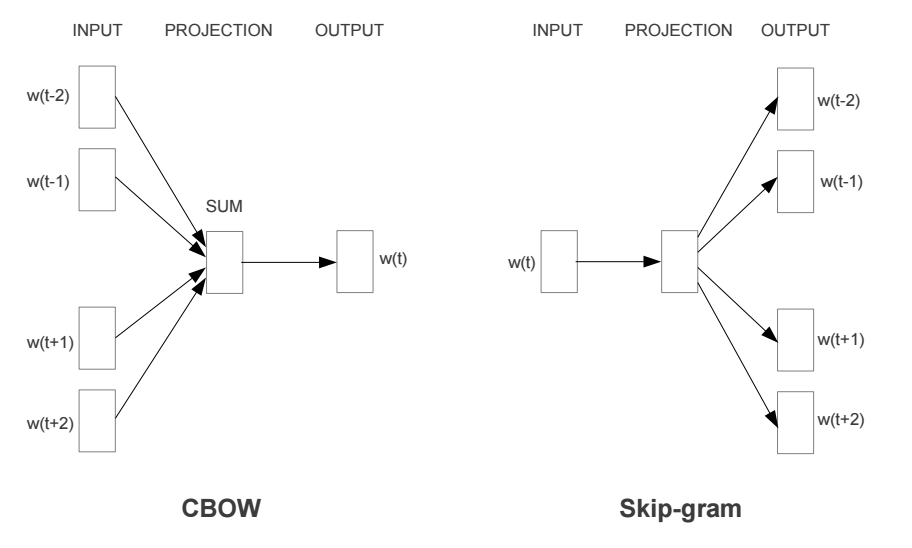
\includegraphics[width=0.75\textwidth]{word2vec} 
   \caption{The two common architectures of word2vec. The Continuous Bag-of-Words (CBOW) model predicts the current word based on the
context, and the Skip-gram predicts surrounding words given the current word. From \cite{mikolov2013efficient}.}
   \label{fig:word2vec}
   \end{center}

\end{figure}


\begin{figure}[h]
\begin{center}
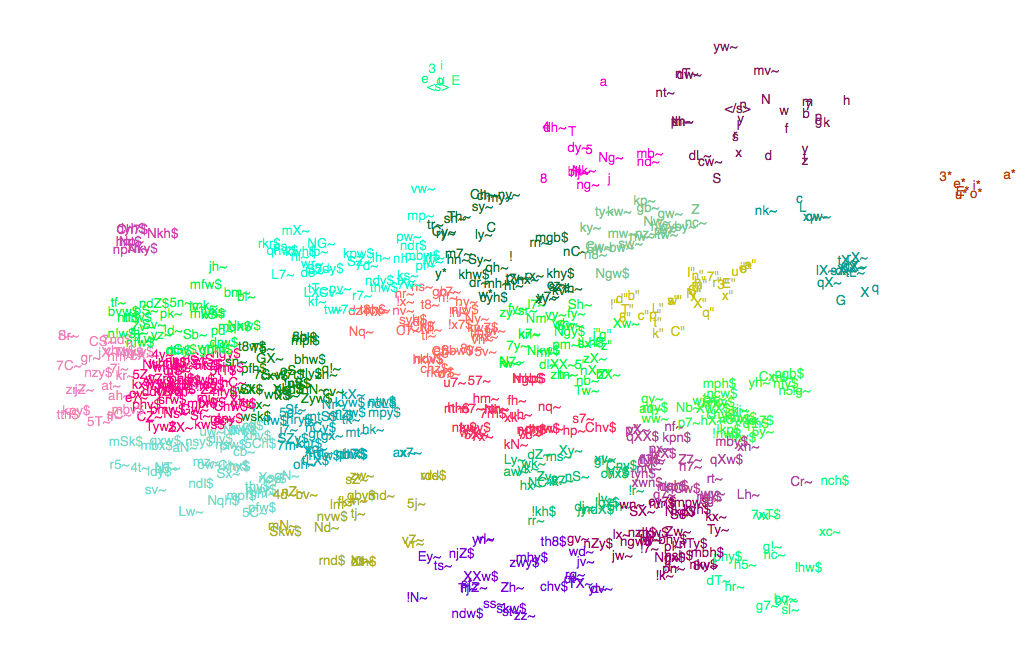
\includegraphics[width=\textwidth]{phoneme_embeddings_overview_ap} 
\caption{t-SNE visualization of the embeddings of all 720 phonemes contained in ASJP, trained with word2vec. The colors represent clusters inferred by Affinity Propagation. The model can clearly separate vowels and various forms of special articulation types. Pulmonic consonants can also be separated clearly from other coarticulation variants, as can uvular or pre-nasalized sounds. Less frequent phonemes, however, cannot be clearly differentiated. }
\label{fig:phoneme_embeddings_overview_ap}
\end{center}
\end{figure}

\begin{figure}[h] %  figure placement: here, top, bottom, or page
   \centering
   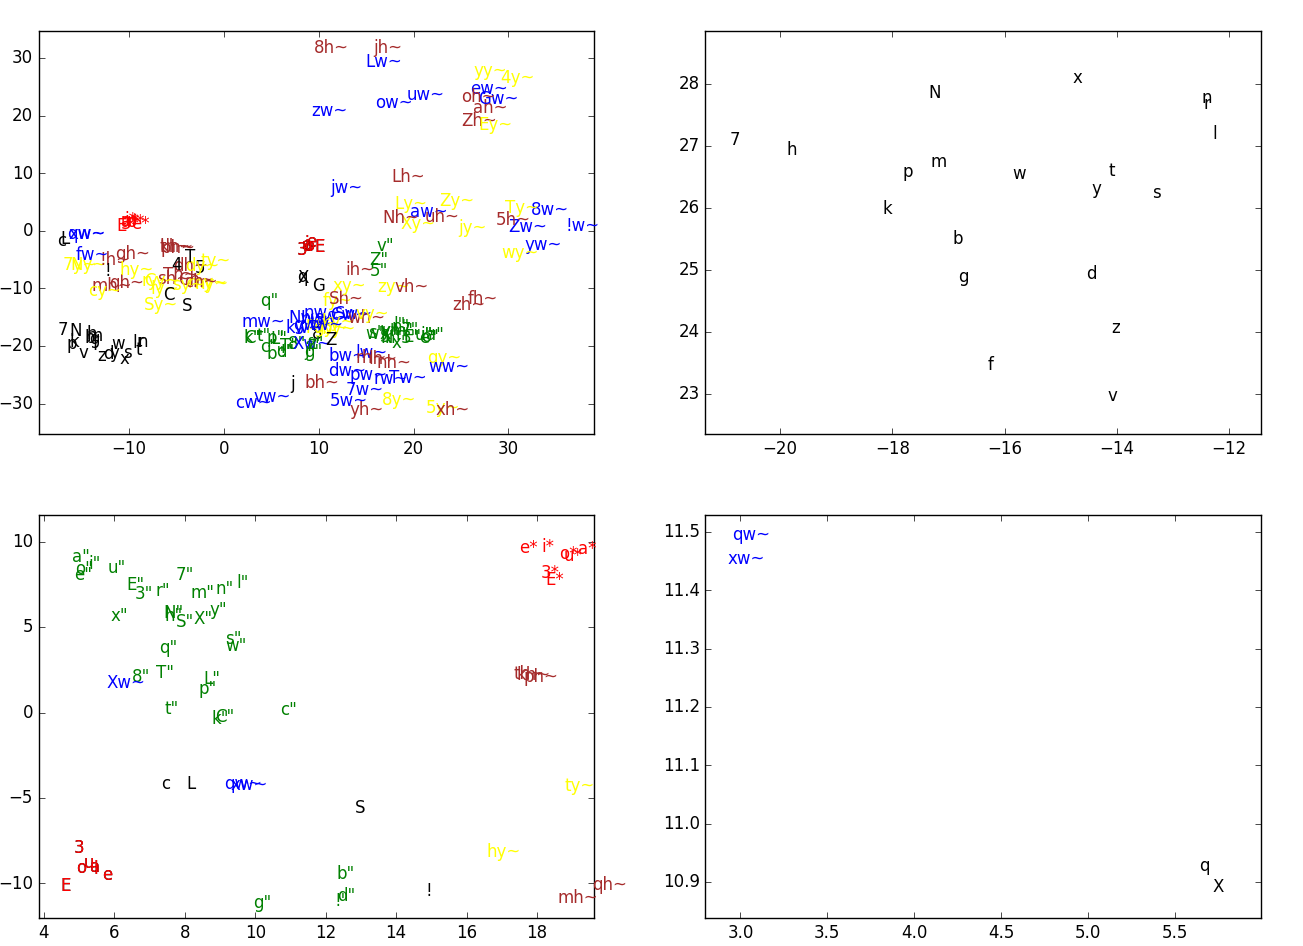
\includegraphics[width=\textwidth]{phoneme_embeddings_word2vec_all} 
   \caption{Other t-SNE visualizations of the embeddings created by word2vec. (top left) The model learns to clearly separate natural classes such as vowels, plain pulmonic or glottalized consonants, while other articulations seem to spread over the feature space. The colors indicate membership of a natural phonological class.  (top right) A more detailed view on plain pulmonic consonants. Note the linear dependencies between voiced and unvoiced plosives and their respective nasal variant. (bottom left) Another detailed view. Note how the labialized uvular sounds cluster among glottalized consonants. (top right) The model seems to capture different manners of articulations across articulation type boundaries, as the linear dependency shows here.}
   \label{fig:phoneme_embeddings_word2vec_all}
\end{figure}

\begin{figure}[h!] %  figure placement: here, top, bottom, or page
   \centering
   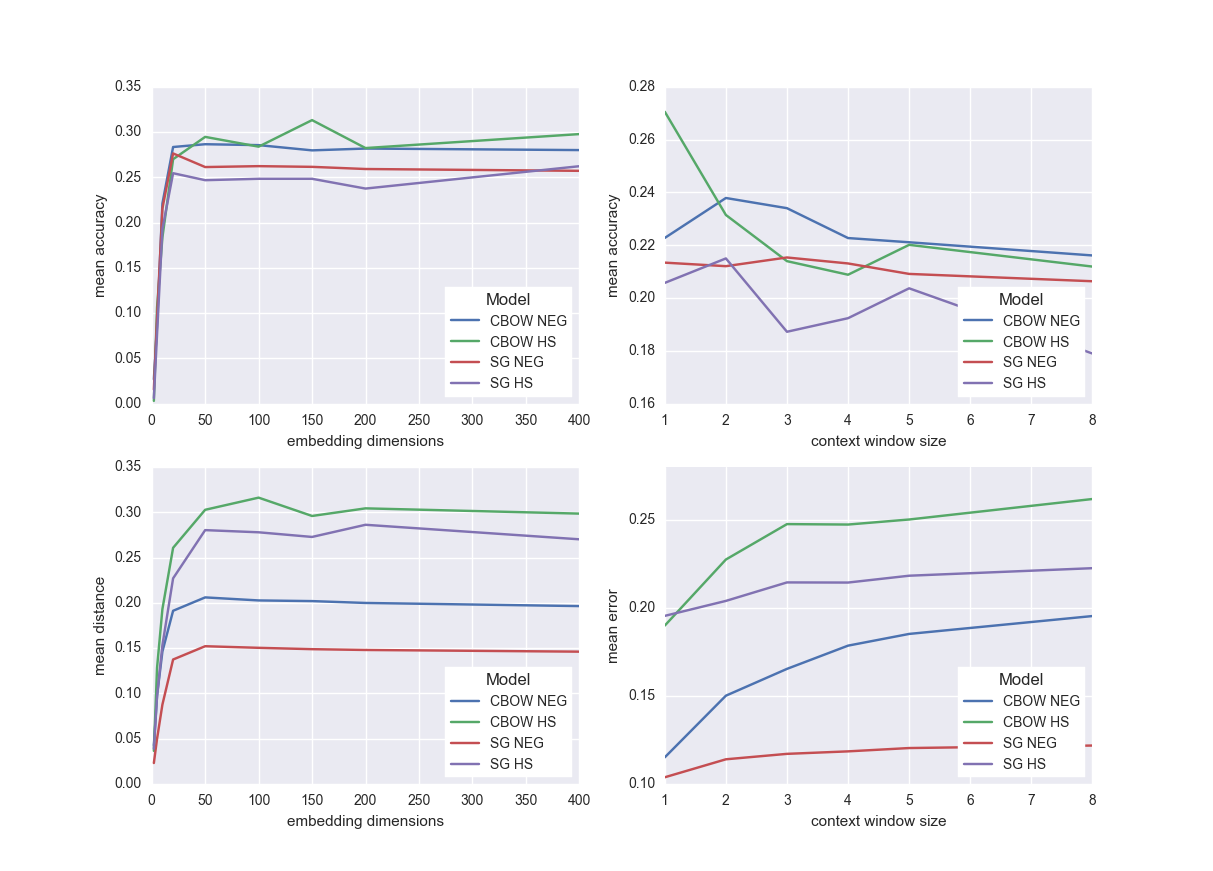
\includegraphics[width=\textwidth]{phoneme_embeddings_4models_comparison_meanAccLossTopn1} 
   \caption{Comparison of the four word2vec models evaluated. (top left) Both CBOW Models perform better than the skip-gram models over all numbers of embedding dimension. (bottom left) Mean distance between the predicted vector and the target with regard to embedding dimensions. Here, negative sampling yields less error than hierarchical softmax. (top right) Mean accuracy for the models with regard to the context window size. The models perform worse the bigger the context is. (bottom right) Mean distance between the predicted vector and the target with regard to context window size. Again, bigger contexts lead to worse predictions. }
   \label{fig:phoneme_embeddings_4models_comparison_meanAccLossTopn1}
\end{figure}

\begin{figure}[h] %  figure placement: here, top, bottom, or page
   \centering
   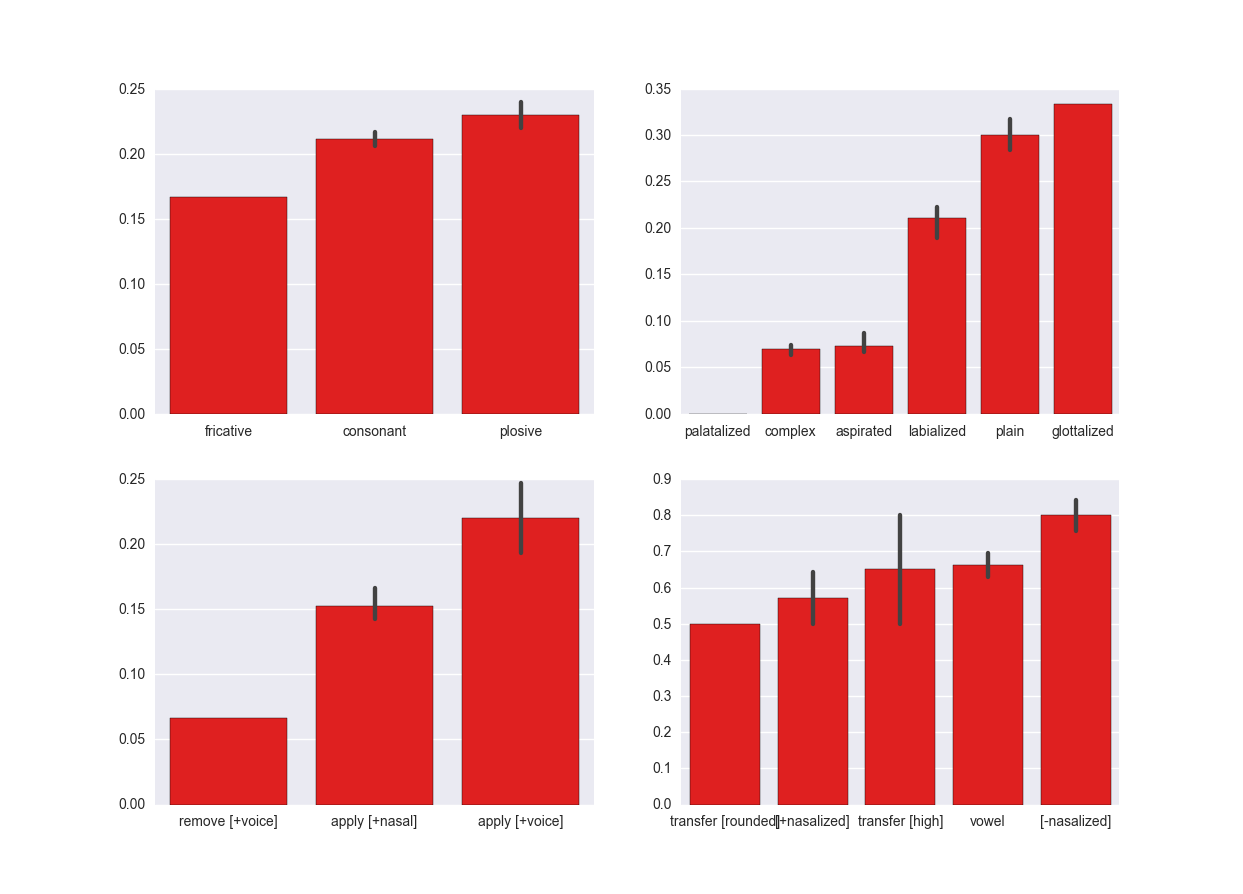
\includegraphics[width=0.75\textwidth]{phoneme_embeddings_detailed_evaluation_topn1} 
   \caption{Mean accuracies for analogies. The model does not seem to be able to capture the compositionality of the latent features too well. (top left) Accuracy is best for plosives across plain pulmonic as well as more complex articulations, while fricatives perform worse. (top right) Glottalized and Plain pulmonic consonant phonemes yield best performance. Among complex articulations, which all perform bad,  labialized phonemes yield best results, while aspirated and palatalized phonemes perform even worse. (bottom left) Adding voice works better than removing it or adding nasality. (bottom right) Vowel analogies work far better than consonant analogies. This should be due to the small number of possible vowel phonemes.}
   \label{fig:phoneme_embeddings_detailed_evaluation_topn1}
\end{figure}

\begin{figure}[h!] %  figure placement: here, top, bottom, or page
   \centering
   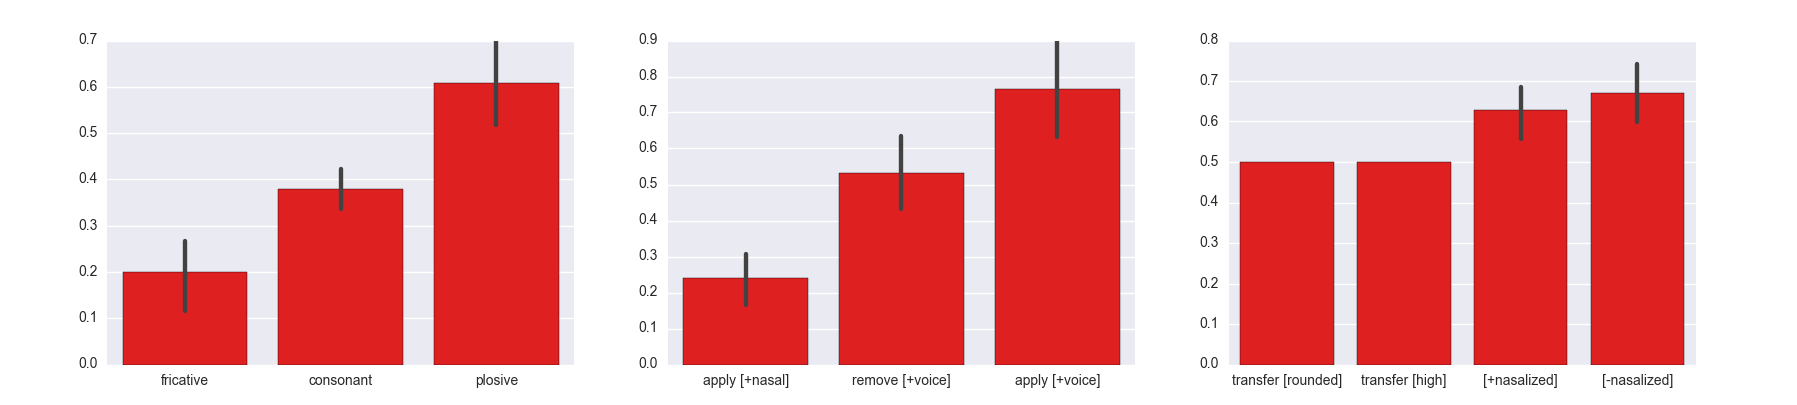
\includegraphics[width=\textwidth]{phoneme_embeddings_detailed_evaluation_consonants_topn1_poooled} 
   \caption{Mean accuracies for analogies over the pooled consonant phonemes. Here, the model is expected to yield better results, as the number of latent features should have been reduced. (left) Accuracy is doubled compared with the unpooled phonemes. (middle) Adding voice works quite well, while removing it still yields acceptable performance. Applying nasality again works quite bad. (right) Vowel analogy tasks seem to work reasonably well, but worse than with unpooled consonants.}
   \label{fig:phoneme_embeddings_detailed_evaluation_topn1_poooled}
\end{figure}


\subsection{Word Embeddings}
\label{Word Embeddings}
\subsubsection{Autoencoders}

Autoencoders are a family of neural network architectures that are trained to construct a code of some given data. Given an encoder function $f: \mathcal{X} \rightarrow \mathcal{Z}$ and a decoder (i.e. generator) function $g: \mathcal{Z} \rightarrow \mathcal{X}$, they are trained on encoding and reconstructing the data, yielding a loss function
\begin{equation}
L(x,g(f(x)))
\end{equation}
 
where $L$ describes some loss function that penalizes the reconstruction error. The dimensionality of $\mathcal{Z}$ is usually assumed to be lower-dimensional, so that autoencoders can be used to reduce the dimensionality of the data. If $f$ and $g$ are linear functions, autoencoders are proven to be equal to PCA. If they are non-linear, they should allow for the detection of latent features.
\subsubsection{Variational Autoencoders}
\label{Variational Autoencoders}
\begin{figure}[h] %  figure placement: here, top, bottom, or page
   \centering
   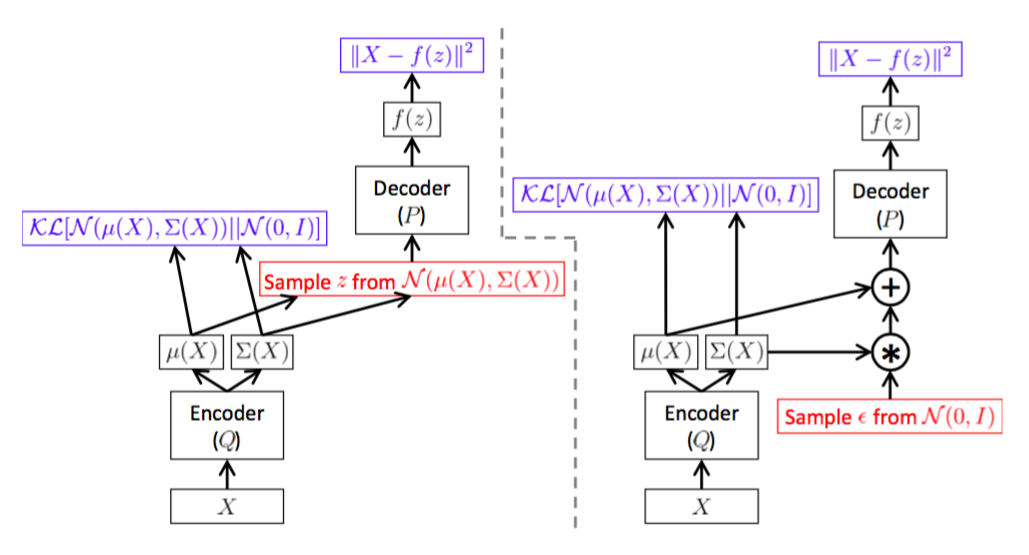
\includegraphics[width=\textwidth]{vae_model_visualization} 
   \caption{Visualization of the Variational autoencoder architecture. (left) The model with original objective as in Eq. \ref{eq:vae_loss_original}. The stochastic unit is inside the network and would not allow for the backpropagation of error gradients through the network. (right) The model after the reparameterization with the objective as in Eq. \ref{eq:vae_loss_reparameterized}. Here, the sampling is interpreted as an input variable, so error gradients can be backpropagated through the whole model. From \cite{doersch2016tutorial}.}
   \label{fig:vae_model_visualization}
\end{figure}

Variational Autoencoders (VAEs) were first described in \cite{kingma2013auto}. Instead of just using a lower-dimensional layer as a bottle neck for non-linear dimensionality reduction, VAEs assume that the code can be modeled by a latent variable $z$ with some prior $p(z)$. This allows for the incorporation of bayesian inference tasks where the marginalization of variables is important, including maximum a posteriori estimates of $\theta$ and an approximation of the posterior $P(z|X)$. Instead of encoder and decoder functions, distributions are used instead to model the relationship between $\mathcal{X} $ and $  \mathcal{Z}$.

As variational models, VAEs do not attempt to sample from the true posterior distribution $P(z|X)$ directly. Markov Chain Monte Carlo methods such as Gibbs sampling or Hamiltonian Monte Carlo rely on whole batches during training, which is not suitable for bigger data sets. Instead, variational method assume that the true posterior can be approximated by another parametric distribution $Q(z|X)$ whose parameters can be estimated analytically. 

In order to approximate the true posterior  $P(z|X)$ with the approximate posterior $Q(z|X)$, we want to minimize the Kullback-Leibler divergence from the true posterior to its approximation: 

\begin{equation}
D_{KL}(Q(z|X)|P(z|X)) = E_{z\sim Q}[\log Q(z|X) - \log P(z|X)]
\end{equation}

Here, we can use Bayes' rule to yield 

\begin{equation}
D_{KL}(Q(z)|P(z|X)) = E_{z\sim Q}[\log Q(z|X) - \log P(X|z)-\log P(z)] + \log P(X)
\end{equation}

where $\log P(X)$ is outside the expectation since it is not dependent on $z$. We can rearrange that to 

\begin{equation}
\label{eq:vae_loss_original}
\log P(X) - D_{KL}(Q(z|X)|P(z|X)) = E_{z\sim Q}[\log P(X|z) - D_{KL}(Q(z|X)||P(z))] 
\end{equation}

Here, the left hand side makes it clear why Eq. \ref{eq:vae_loss_original} is to be maximized, as it increases the probability of $X$ and minimizes the divergence from the true to the approximated posterior. We further have $Q(z|X)$ as an \textit{encoder} that maps data points into the latent space $\mathcal{Z}$ and $P(X|z)$ as a \textit{decoder} that reconstructs a data point, given a sample $z$. As the universal approximation theorem states that networks with at least one hidden layer can approximate any continuous functions, we can reduce $D_{KL}(Q(z|X)||P(z|X))$ to zero and optimize $P(x)$ directly. The right hand side is the \textit{variational lower bound} that defines the probability that the encoder distribution $Q(z|X)$ approximates the true prior $P(z)$ and then $z$ is decoded back to it initial value in $\mathcal{X}$.

To estimate the parameters of $Q$,  \cite{kingma2013auto} propose Multilayer Perceptrons (MLPs) as universal function approximator.

However, given that we use neural networks, we have to make sure that all gradients can be backpropagated through the network. In Eq. \ref{eq:vae_loss_original}, moving the gradient symbol into the expectation on the right hand side would yield gradients that would be independent of the parameters of $Q$. This is due to the location of the sampler as a unit inside the network - since sampling from $Q(z|X)$ is a non-continuous operation, it cannot have gradients and hence would block the backpropagation of errors to the encoder network. \cite{kingma2013auto} instead propose another objective that treats the sampling as an input to the network: Here, an auxiliary noise variable $\epsilon$ is sampled from some distribution $p(\epsilon)$:

\begin{equation}
\epsilon \sim p(\epsilon)
\end{equation}

\cite{kingma2013auto} mention that  $p(\epsilon)$ can be any continuous distribution or compositions of such distributions, but propose to use a standard normal distribution if $z$ is model by a normal distribution:
\begin{equation}
\epsilon \sim \mathcal{N}(0,1)
\end{equation}

With $\epsilon$ at hand, we can reformulate $z$ as a deterministic variable:
\begin{equation}
z = \mu + \sigma \odot \epsilon
\end{equation}

The right hand side of Eq. \ref{eq:vae_loss_original} then becomes
\begin{equation}
\label{eq:vae_loss_reparameterized}
E_{\epsilon \sim \mathcal{N}(0,1)}[\log P(X|z= \mu + \sigma \odot \epsilon) - D_{KL}(Q(z|X)||P(z))] 
\end{equation}

The model architecture is visualized in Fig. \ref{fig:vae_model_visualization}. 

%VAEs first draw a sample from $p(z)$. That code than runs through a differentiable generator network $g(z)$. $x$ is then finally sampled from the likelihood $p(x;g(z)) = p(x|z)$ (cf. \cite[p. 698]{Goodfellow-et-al-2016-Book}) 
%
%The model learns to maximize the variational lower bound $\mathcal{L}(\theta,\phi,x^{(i)})$.
%
%\begin{equation}
%\log p_\theta(x^{(i)}) = D_{KL}(q_{\phi}(z|x^{(i)})||p_\theta(z|x^{(i)}))+\mathcal{L}(\theta,\phi,x^{(i)})
%\end{equation}
%
%where the first term on the right is the Kullback Leibler Divergence of the approximated posterior to the true posterior, while the second therm is the variational lower bound on the marginal likelihood of the datapoint i.
%
%
%Given the probabilistic encoder $q_{\phi}(z|x)$, which serves as the approximation to the posterior of the model $p_{\theta}(z,x)$, we have a prior
%
%\begin{equation}
%p_{\theta}(z) = \mathcal{z;0,I} 
%\end{equation}
%
%The probabilistic decoder $p_{\theta}(x|z)$ can be a multivariate Gaussian or a Bernoulli distribution, depending on the data. The respective distribution parameters are inferred from z with a Multilayer Perceptron (MLP). The variational approximate posterior is then given by  
%
%
%\begin{equation}
%\log q_{\phi}(z|x^{(i)}) = \log \mathcal{N}(z;\mu ^{(i)},\sigma ^{2(i)}I)
%\end{equation}
%
%where $\mu$ and $\sigma^2$ are inferred by the encoding MLP. 

%\begin{equation}
%\mathcal{L}(\theta,\phi,x^{(i)}) \simeq \frac{1}{2} \sum_{j=1}^{J}(1+\log((\sigma_j^{(i)})^2 )-(\mu_j^{(i)})^2 -(\sigma_j^{(i)})^2)
%+ \frac{1}{L}\sum_{l=1}^L \log p_{\theta}(x^{(i)}|z^{(i,l)})
%\end{equation}
%
%where 
%
%\begin{equation}
%z^{(i,l)} = \mu(i) + \sigma^{(i)} \odot \epsilon^{(l)}
%\end{equation}
%
%and 
%
%\begin{equation}
%\epsilon^{(l)} \sim \mathcal{N}(0,I)
%\end{equation}

For practical purposes, such a model should not take too much time to learn the relationships between the words in our wordlist. 

Following this, 2 different models are investigated here:
\begin{enumerate}
\item A model that tries to maximize $P(X|z)$, i.e. that learns the manifold creating the words as such. Such as model is pre-trained on a big corpus of phonologically annotated words. Here, the assumption is that if we embed our word list, we can use the maximum likelihood assumption that states that if the training data is representative for the data as such, it should be able to generalize well for similar, but unseen data. This model will be referred to as VAE-PT.
\item A model that tries to maximize $P(X|z,C)$, i.e that learns the manifold creating words given the respective concept. Such a model is useful as we are only interested to cluster words given a concept class. Also, this means that we only look for latent features in a given semantic concept, which should allow for finer-grained latent features. This model will be referred to as VAE-C.
\end{enumerate}

\subsection{Clustering}

To cluster the embeddings, we have to make sure that the number of clusters can vary, as can the number of members for each cluster. For instance, if our word list consists of languages where the majority of languages are closely related and should show similar words, but the remaining languages are not related at all, we assume that the resulting clusters of words are not of the same size. If we do not know at all if the respective languages are related, we cannot really say what size the clusters should have either. Hence, both are variables which we do not know beforehand. 

This thesis proposes Affinity propagation (cf. \cite{frey2007clustering}) to solve that task. Here the algorithm exchanges real-valued messages between the data points until a high-quality set of exemplars and corresponding clusters
gradually emerges. This allows for the number of clusters and individual cluster size to be left undefined.

As we know that  certain subspaces in $\mathcal{Z}$ accumulate more probability mass than others, we can assume that this should affect the similarity between points in $\mathcal{Z}$. In fact, the group of words with low self-information cluster among each other and are probably even closer to each other than members of actual cognate classes. Hence we have to weight the distances between the embeddings according to their respective self-information.

We can define this distances as 

\begin{equation}
d_{weighted}(z_1,z_2) = d_{euclidean}(\frac{z_1}{I(z_1)}),\frac{z_2}{I(z_2)}))
\end{equation}

This means that the lower the self-information for a given word is, the farer its position is shifted away from its current position. If two embeddings are close to each other but have low self-information, the weighted distance between them is correspondingly larger than the actual euclidean distance. However, if the self-information is bigger, the words can reside in a cluster with higher variance, but the weighted distance between them would be smaller than if that cluster would be situated in an area with high probability mass.


\section{Evaluation}
\subsection{Data}
To pre-train VAE-PT,  the data provided by the Automatic Similarity Judgement Program (ASJP, \cite{wichmann2010asjp} will serve as a training corpus. ASJP provides wordlists of roughly 7200 languages, where each word is given as a string of phonemes. This vast amount of different phoneme inventories will allow for the unbiased comparison of phonemes over language boundaries. However, ASJP does not make use of IPA, but a simplified phonemic alphabet that is based on ASCII-characters. This makes it possible to incorporate data where no detailed IPA description is given, but might also reduce the quality of the resulting embedding space, as latent features that might be encoded in more specific IPA descriptions are merged. For all other data, respective conversions into the ASJP system are used.  An overview of the ASJP phonemes and their IPA counterparts are given in the appendix.

Both models are tested on IELex (cf. \cite{dunn2012indo}) and the 
\subsection{Evaluation of $P(X)$}

A first visual inspection shows that the model learns to cluster similar strings close to each other (Fig. \ref{fig:vae_phono_binary_asjp_subsample_words}). Words with similar syllable structures are located in specific subspaces of $\mathcal{Z}$. It further connects strings beyond local clusters through linear dependencies, which can interchange whole syllables of a word. 
On a more global perspective, words are embedded into a high-level feature continuum that encodes word lengths (Fig. \ref{fig:vae_phono_binary_wordLength}), with smooth transitions between the respective subspaces. This is remarkable, given that there are no word boundary tokens involved during training. The model itself learns to recognize the transition from the binary code of the actual phonemes of the word to the zero-padding following it.
Moreover, the linear dependencies are not simple renderings of the binary input code. The model learns high-level latent features, such as if a word has a phoneme with a certain distinctive feature or not (Fig. \ref{fig:vae_phono_binary_features}). If so, linear dependencies connect such words, even over very long distances. In fact, some of those linear dependencies form bigger clusters that can span the entire posterior distribution. 
Even more remarkable is that the model learns to cluster words with similar coarticulation features \textit{even though they were excluded during training}, but only existent on some latent level (Fig. \ref{fig:vae_phono_orthofeatures}). Here, the model learns to distinguish plain /w j h/ from true labialization, palatalization and aspiration, although they were merged in the input code. If the model treated them as equal, we would expect a uniform distribution over the respective words. However, we see that the words accumulate in different subspaces. Since the model learns to cluster words according to their phonological structure, it recognizes that the context plain /w j h/ occur in differs from the context of coarticulated phonemes and hence locates the respective words in different subspaces of $\mathcal{Z}$.

\begin{figure}[h] %  figure placement: here, top, bottom, or page
   \centering
   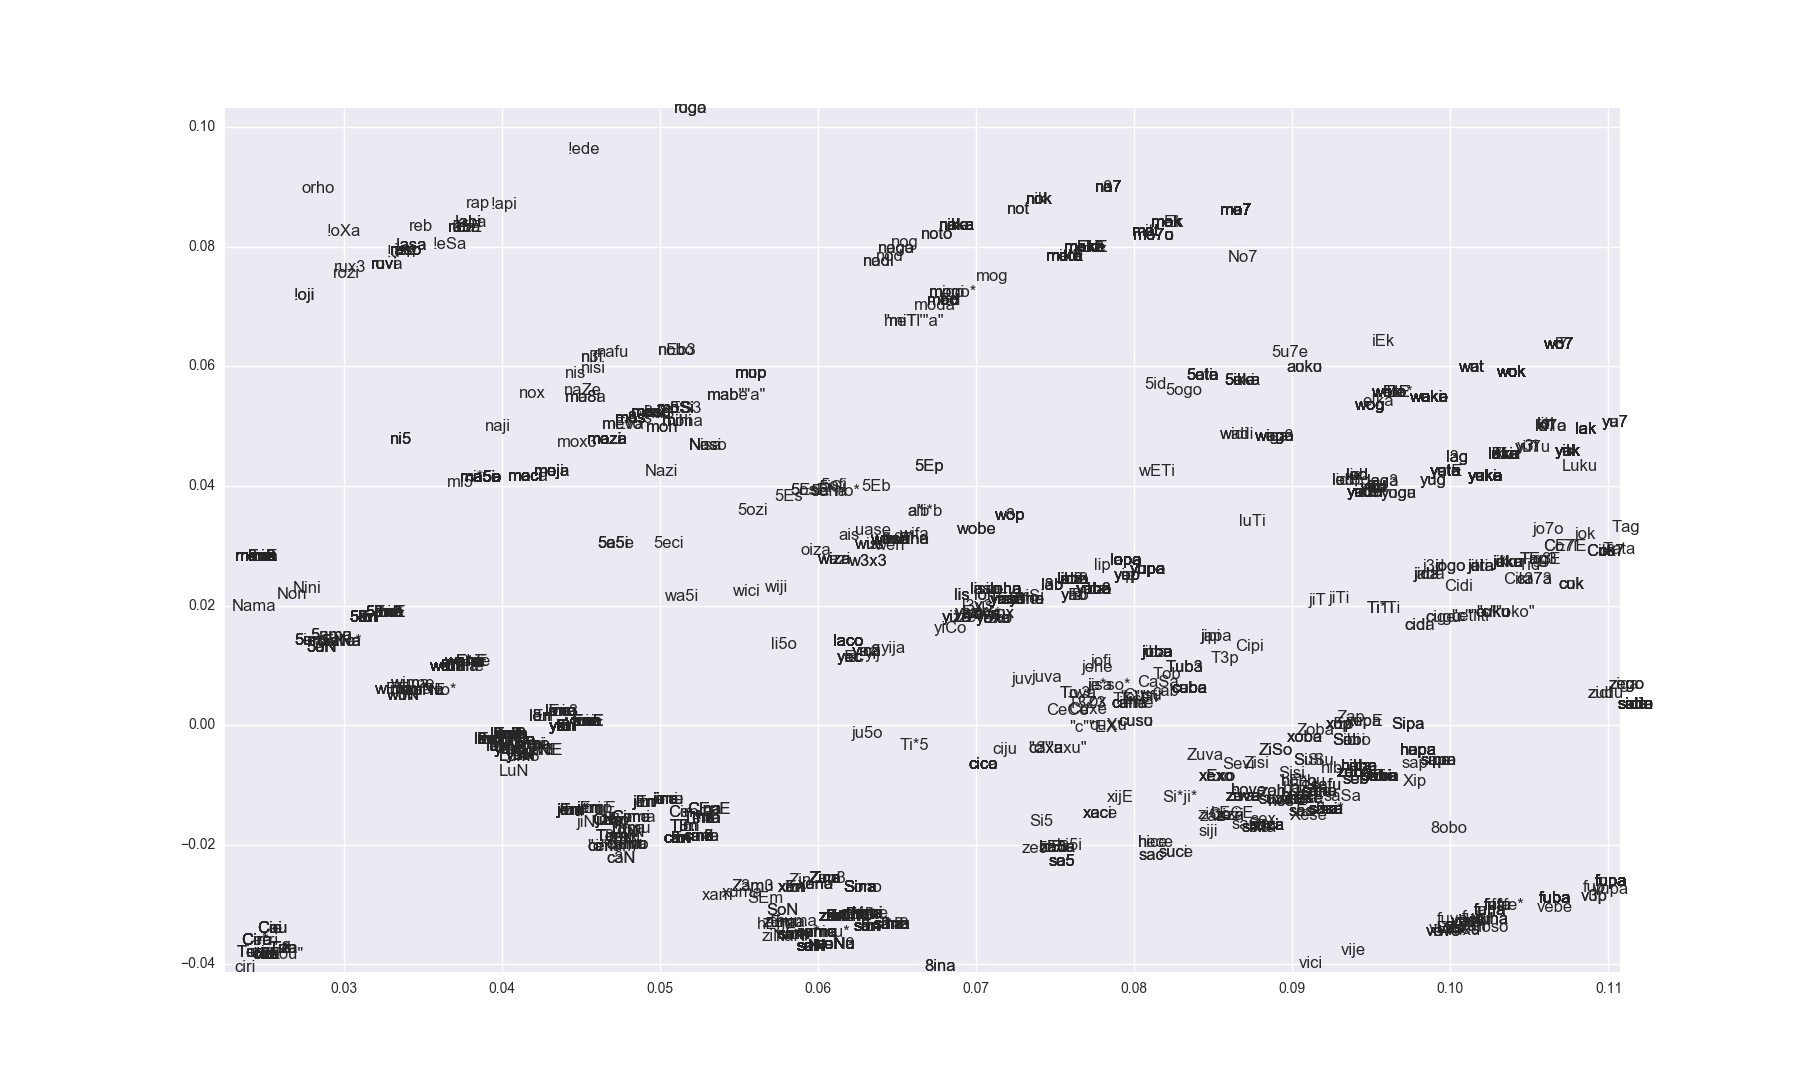
\includegraphics[width=\textwidth]{vae_phono_binary_asjp_subsample_words} 
   \caption{A detailed view on a subsample of ASJP embedded into $\mathcal{Z}$ after trained on the whole ASJP data set for 100 iterations. As can be seen, words accumulate in local subspaces with higher probability mass. Here, all words are contained in an area with shorter words that show simple CV syllable structures. Words that only differ in one distinctive feature are very close to each other, while linear dependencies over longer distances signify relationships over whole syllables that are exchanged.}
   \label{fig:vae_phono_binary_asjp_subsample_words}
\end{figure}

    
    \begin{figure}[ht] 
  \begin{subfigure}[b]{0.5\linewidth}
    \centering
    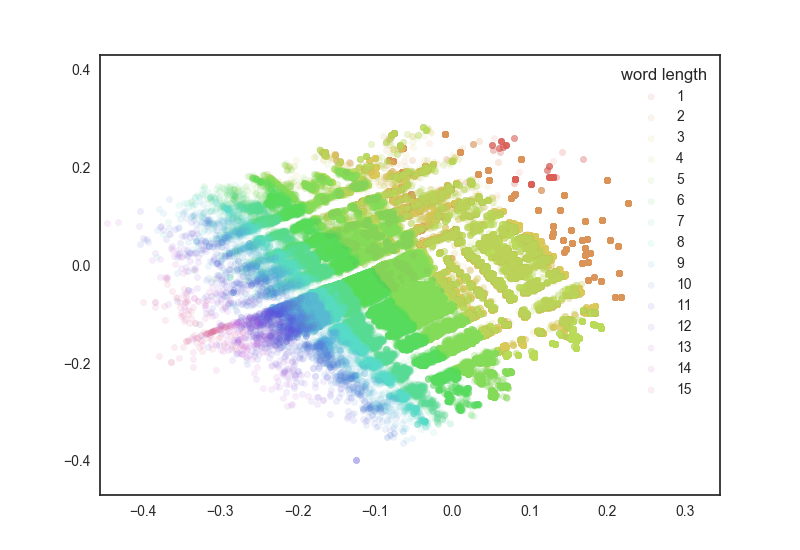
\includegraphics[width=\linewidth]{vae_phono_binary_wordLength} 
    \label{fig:vae_phono_binary_wordLength0} 
    \vspace{4ex}
  \end{subfigure}%% 
  \begin{subfigure}[b]{0.5\linewidth}
    \centering
    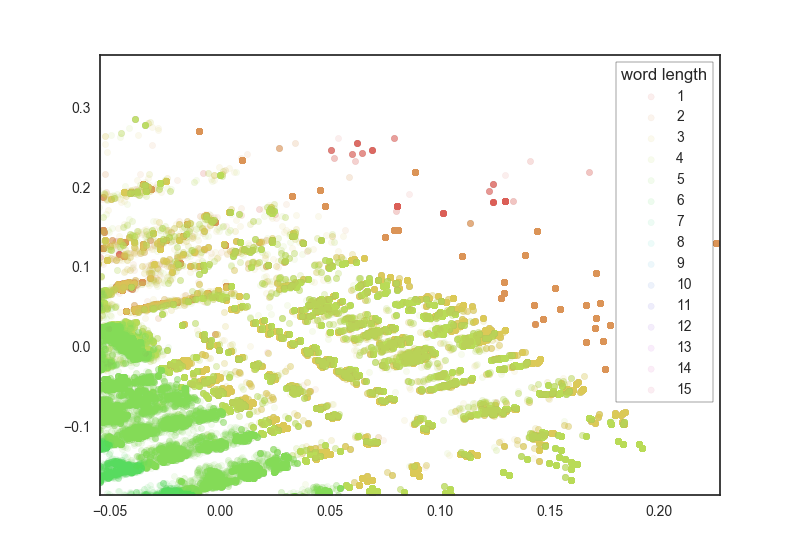
\includegraphics[width=\linewidth]{vae_phono_binary_wordLength_detail1} 
    \label{fig:vae_phono_binary_wordLength1} 
    \vspace{4ex}
  \end{subfigure} 
  \begin{subfigure}[b]{0.5\linewidth}
    \centering
    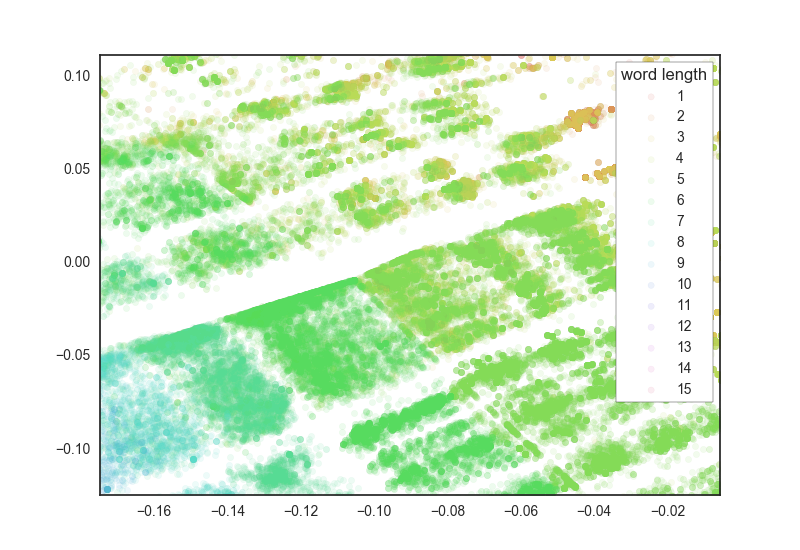
\includegraphics[width=\linewidth]{vae_phono_binary_wordLength_detail2} 
    \label{fig:vae_phono_binary_wordLength2} 
  \end{subfigure}%%
  \begin{subfigure}[b]{0.5\linewidth}
    \centering
    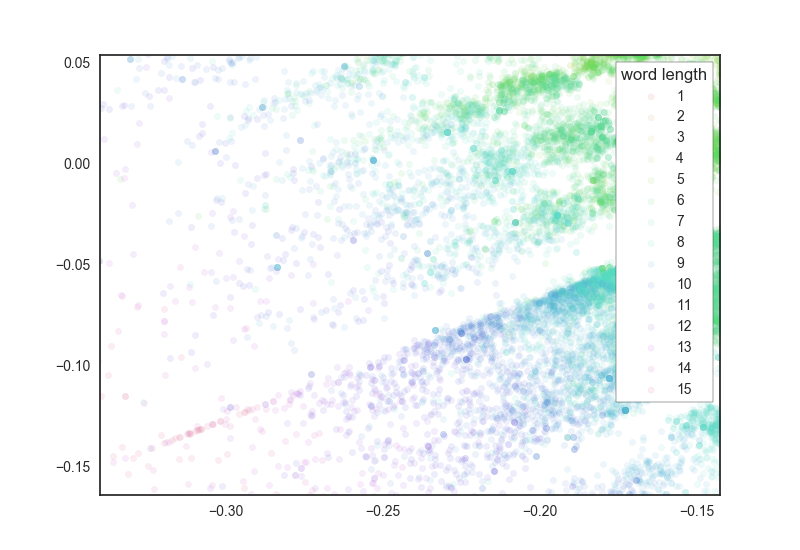
\includegraphics[width=\linewidth]{vae_phono_binary_wordLength_detail3} 
    \label{fig:vae_phono_binary_wordLength3} 
  \end{subfigure} 
  \caption{The ASJP data set embedded into $\mathcal{Z}$ after trained on it for 100 iterations, colored by word length. The model learns to cluster words according to their respective length, with more frequent word lengths located in subspaces with higher probability mass.}
  \label{fig:vae_phono_binary_wordLength} 
\end{figure}

    \begin{figure}[ht] 
  \begin{subfigure}[b]{0.5\linewidth}
    \centering
    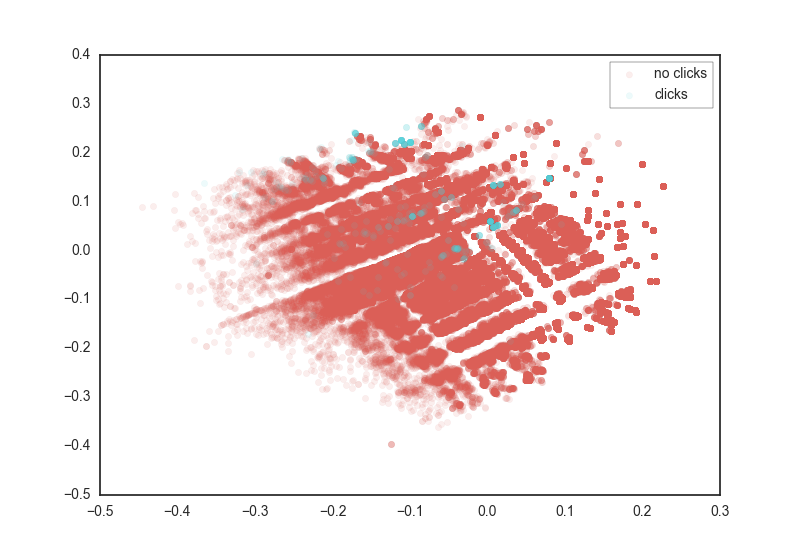
\includegraphics[width=\linewidth]{vae_phono_binary_clicks} 
    \label{fig:vae_phono_binary_features0} 
    \vspace{4ex}
  \end{subfigure}%% 
  \begin{subfigure}[b]{0.5\linewidth}
    \centering
    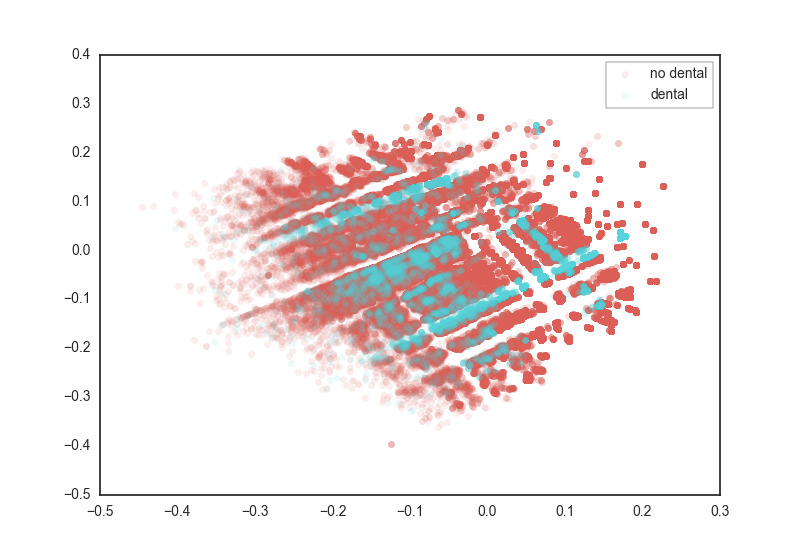
\includegraphics[width=\linewidth]{vae_phono_binary_dental} 
    \label{fig:vae_phono_binary_features1} 
    \vspace{4ex}
  \end{subfigure} 
  \begin{subfigure}[b]{0.5\linewidth}
    \centering
    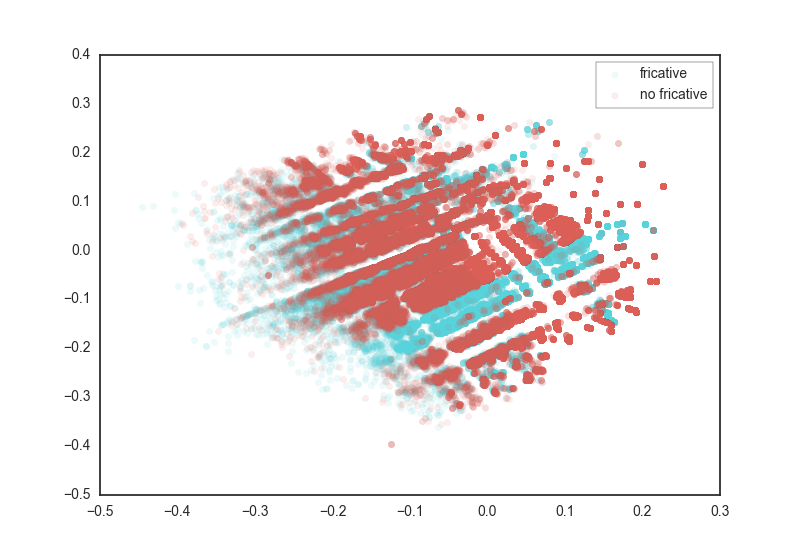
\includegraphics[width=\linewidth]{vae_phono_binary_fricative} 
    \label{fig:vae_phono_binary_features2} 
  \end{subfigure}%%
  \begin{subfigure}[b]{0.5\linewidth}
    \centering
    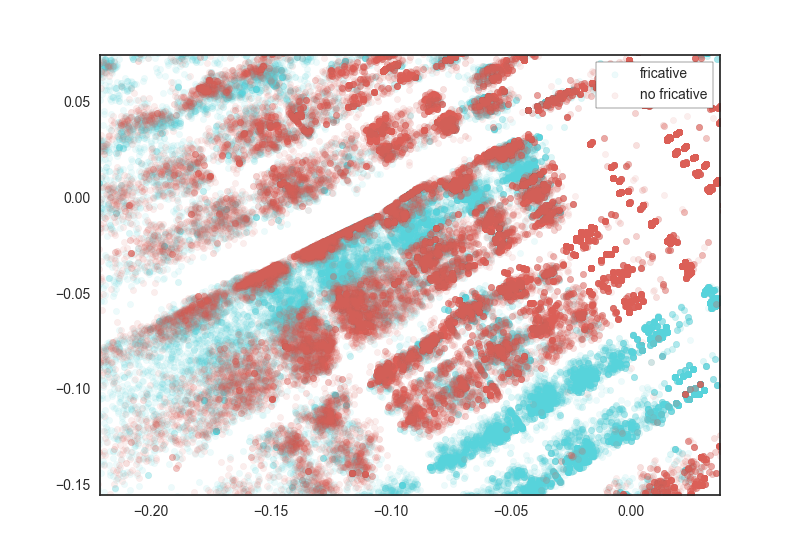
\includegraphics[width=\linewidth]{vae_phono_binary_fricative_detail1} 
    \label{fig:vae_phono_binary_feature3} 
  \end{subfigure} 
  \caption{The ASJP data set embedded into $\mathcal{Z}$ after trained on it for 100 iterations, colored by whether a given word has a phoneme with some specific distinctive feature. (top left) The model learns that clicks are highly unlikely to emerge evolutionary and hence assigns low probability mass to their respective subspace. (top right) The distribution of words with and without dentals. The linear dependencies are clearly visible. (bottom left) The distribution of words with and without fricatives. Again, it can be seen how they are linearly dependent of each other. (bottom right) A detailed view on the words with and without fricatives.}
  \label{fig:vae_phono_binary_features} 
\end{figure}

    \begin{figure}[ht] 
  \begin{subfigure}[b]{0.5\linewidth}
    \centering
    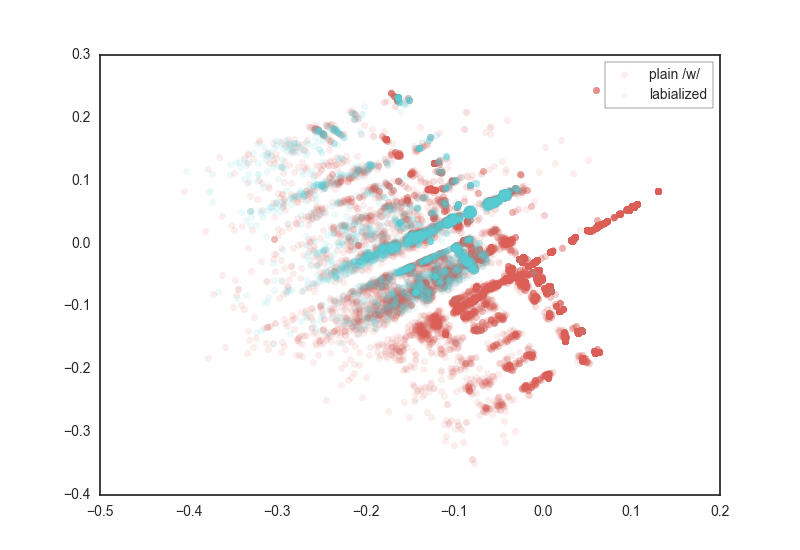
\includegraphics[width=\linewidth]{vae_phono_binary_orthofeature_labialized} 
    \label{fig:vae_phono_orthofeatures0} 
    \vspace{4ex}
  \end{subfigure}%% 
  \begin{subfigure}[b]{0.5\linewidth}
    \centering
    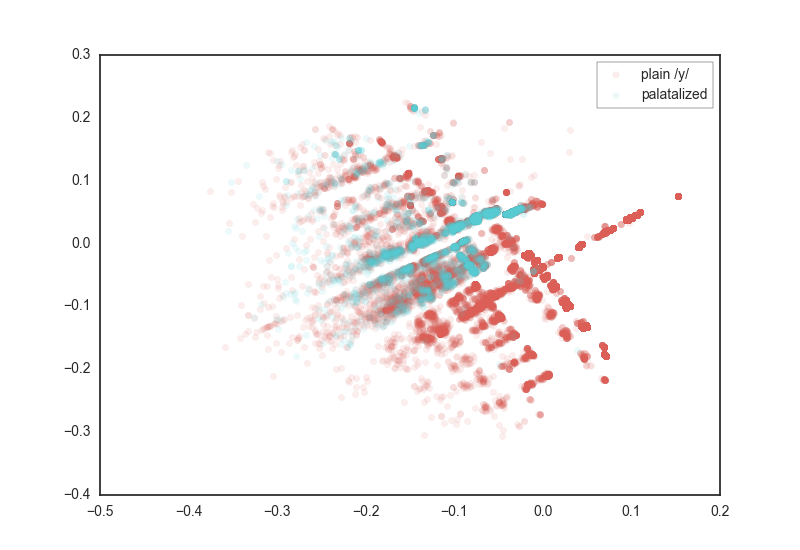
\includegraphics[width=\linewidth]{vae_phono_binary_orthofeature_palatalized} 
    \label{fig:vae_phono_orthofeatures1} 
    \vspace{4ex}
  \end{subfigure} 
  \begin{subfigure}[b]{0.5\linewidth}
    \centering
    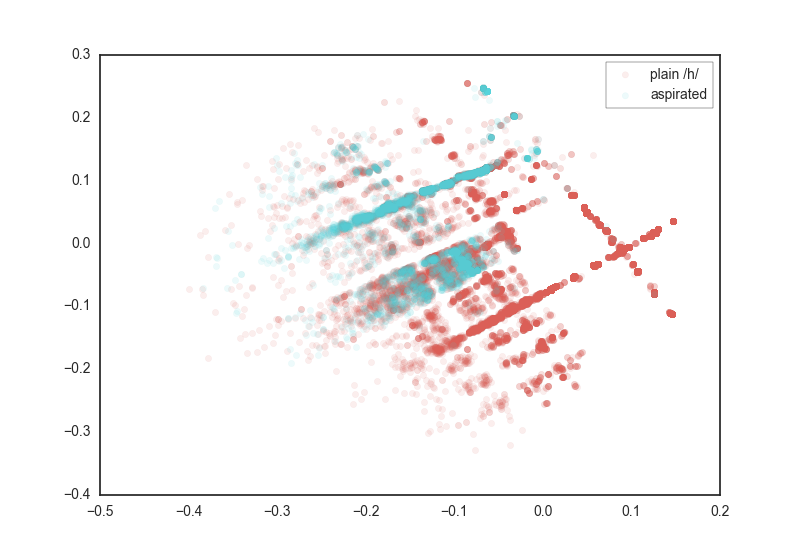
\includegraphics[width=\linewidth]{vae_phono_binary_orthofeature_aspirated} 
    \label{fig:vae_phono_orthofeatures2} 
  \end{subfigure}%%
  \begin{subfigure}[b]{0.5\linewidth}
    \centering
    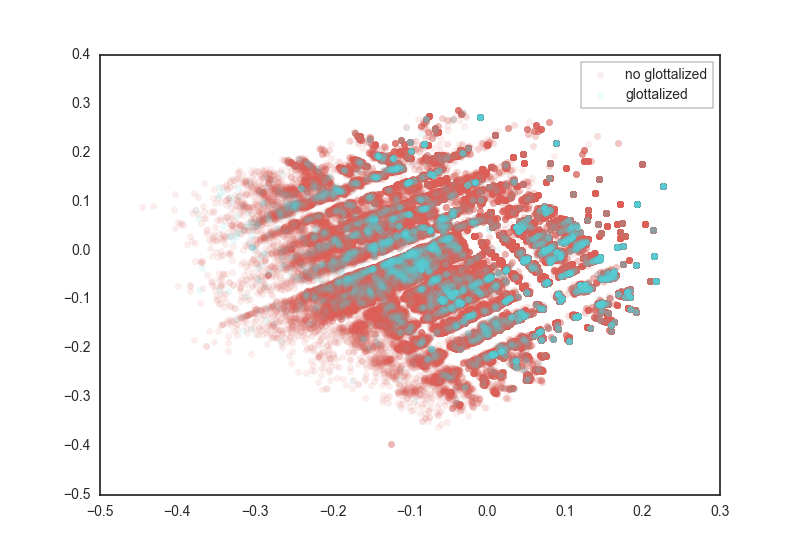
\includegraphics[width=\linewidth]{vae_phono_binary_orthofeature_glottalized} 
    \label{fig:vae_phono_orthofeatures3} 
  \end{subfigure} 
  \caption{The ASJP data set embedded into $\mathcal{Z}$ after trained on it for 100 iterations. Since the binary features ignore coarticulations as such and encode them as independent phonemes instead, the model might learn to distinguish them, given some underlying latent features. (top left) The distribution of words that contain plain /w/ versus words with proper labialization. If the model did not learn the difference, we would expect some uniform distributions over all words that contain /w/ in the input. However, we can clearly see that words with proper labialization are located in other subspaces than words with proper /w/. Moreover, we see that words with labialized phonemes show linear dependence. (top right) The distribution of words that contain plain /y/ versus words with proper palatalization. Again, we see a clear distinction between the two. (bottom left) The distribution of words that contain plain /h/ versus words with proper aspiration. Again, we see a clear distinction between the two. (bottom right) The distribution of words that contain glottalized sounds versus that of words without. As glottalization can cover both vowels and consonants, the distributions are spread over the whole population. However, we can see that glottalized sounds cluster at the bottom right, a subspace containing mostly mostly words with velar and uvular consonants.}
  \label{fig:vae_phono_orthofeatures} 
\end{figure}

\subsection{Results}
\section{Resume}
\section{Acknowledgements}
For training the phoneme embeddings, I used the word2vec implementations provided by the gensim package \cite{rehurek_lrec}. The Autoencoder was implemented with Keras \cite{chollet2015keras} and Tensorflow \cite{tensorflow2015-whitepaper}. The clustering algorithms used here were provided by scikit-learn \cite{scikit-learn}. All code connected to this thesis can be found on my github \footnote{https://github.com/marlonbetz/BA}
%\subsection{}


\bibliographystyle{apa}
\bibliography{references}
\end{document}  